Pode-se observar o esquema do espectrômetro na Figura \ref{fig:tof}, onde o pulso elétrico fornece velocidade perpendicular ao feixe de partículas carregadas, que então viajam dentro de um tubo de voo - livre de variação de potencial elétrico - até encontrarem um detetor de corrente. Por sua vez, o detetor faz a contagem de íons em função dos tempos de chegada.

O TOFMSs funciona  baseado no fato de que, ao receber a mesma quantidade de energia fornecida por um campo elétrico pulsado, partículas com massas/carga diferentes adquirem velocidades distintas \cite{dissertacao_kevin}. Assim, as partículas mais leves atingirão o detector antes das partículas mais pesadas.

\begin{figure}
  \centering
  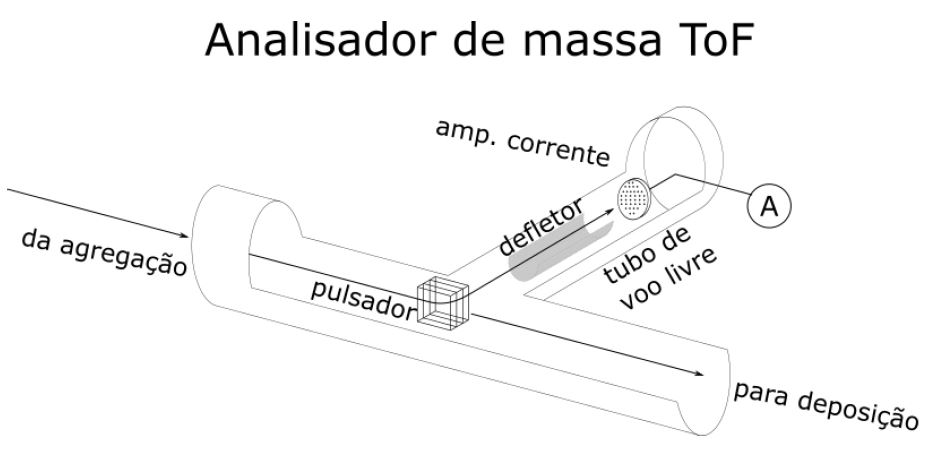
\includegraphics[width=1\textwidth]{images/foca/tof}
  \caption{ O pulsador é um conjunto de placas com campo pulsado, que confere uma velocidade perpendicular ao feixe de partículas eletricamente carregadas. Os defletores impedem que as partículas colidam com as paredes do tubo de voo livre. ``\textit{A}'' representa o detector de corrente, cuja função é realizar a contagem dos íons em função do tempo de chegada.  \cite{dissertacao_kevin}.  }
  \label{fig:tof}
\end{figure}

Para calcular o tempo de voo, vamos considerar um \textit{cluster} de massa $m$ e carga $q$. O campo elétrico vai fornecer energia cinética ($K = qV$) para a partícula, em que $V$ é a voltagem fornecida pelo pulsador. Assim, é possível expressar a velocidade da partícula como:

\begin{equation}
v = \sqrt[]{\frac{2qV}{m}}
\end{equation}

O detector de corrente está situado a uma distância $L$ da região onde a partícula adquire velocidade. Note que essa partícula levará um tempo $t_{voo}$ para atingir o detector, e esse tempo pode ser calculado por:

\begin{equation}
\label{eq:tempo_voo}
t_{voo} = L \cdot \sqrt[]{\frac{1}{2V}}  \sqrt[]{\frac{m}{q}} 
\end{equation}


A corrente que chega ao detector é convertida em tensão por um amplificador IV, e o sinal é exibido em um osciloscópio e, então, para aquisição dos dados utiliza-se um programa desenvolvido pelo grupo.

A variável $L$ possui o valor de um metro, o potencial aplicado é de $V = 7 $  kV, e o tempo de voo das partículas é fornecido pelo osciloscópio, possibilitando calcular a massa das partículas.

Note que utilizando a Equação \ref{eq:tempo_voo} é possível também calcular o $t_{voo}$ de uma partícula se soubermos a massa. Vamos fazer uma análise para o caso de um átomo de prata. Segundo a tabela periódica, um átomo de prata possui uma massa de $107,87$ unidades de massa atômica e convertendo sua massa para quilos, temos $1,79\times 10^{-25}$ kg. A carga de partícula é a carga elementar de um elétron $1,60\times 10^{-19}$ C, e então seu tempo de voo vai ser aproximadamente$17,6$ $\mu$s.

Podemos também escrever a massa de uma nanopartícula em função da massa de uma outra partícula da qual conhecemos a massa e o tempo de voo.

\begin{equation}
\label{eq:relacao_massa_tempo}
M = \left(\frac{t}{t'}\right)^2 \cdot M'
\end{equation}


É possível estabelecer uma relação que futuramente vai permitir diferenciar outros picos de prata, e então calibrar o espectro de partículas produzido, confirmando o que foi depositado na amostra.


A grande vantagem desse tipo de técnica, espectrometria de massa por tempo de voo, é que a obtenção da distribuição de tamanhos das nanopartículas produzidas é exibida em tempo real, assim qualquer variação indesejável no espectro é passível de correção, ainda durante o processo de deposição, por meio de ajuste  dos parâmetros da máquina. 
